%Document type
\documentclass[10pt]{extarticle}

\usepackage[
margin=2.54cm
%,showframe
]{geometry} %package para configurar a geometria base das páginas
\usepackage[table,xcdraw]{xcolor}
\usepackage[portuguese]{babel} %package para o latex usar a lingua portuguesa
\usepackage[utf8]{inputenc} %package dos acentos e assim
\usepackage[T1]{fontenc} %package para existir hifenização correcta em passagens de linha
\usepackage{libertine} %package para usar a font Libertine
\usepackage[hyphens]{url} %package para criar line breaks nos urls, com parâmetro para reconhecer hífenes
\usepackage[hidelinks,linktocpage]{hyperref} %package para poder criar hyperlinks/urls no PDF
\usepackage{graphicx} %package para usar figuras
\usepackage{float} %package para meter à força tabelas e figuras no sítio certo
\usepackage{amsmath} %package para usar o ambiente de matemática
\usepackage{tcolorbox} %package para criar caixas de texto coloridas
\usepackage{fancyhdr} %package para modificar header, footer, page number, etc.
\usepackage{enumitem} %package para configurar os parâmetros dos items num ambiente do tipo itemize
\usepackage{changepage} %package para poder modificar a largura de páginas específicas
\usepackage{eurosym} %package para poder usar o simbolo do euro com especificações de design correctas
\usepackage{textcomp} %package para ter acesso a inúmeros símbolos não nativos ao latex
\usepackage{threeparttable} %package para poder criar footnotes em tabelas
\usepackage{caption} %package para configurar as captions
\usepackage{subcaption} %package para configurar as subcaptions
\usepackage{listings} %package para interpretar código doutras linguagens
\usepackage{multirow} %package para ter tabelas com parâmetros que ocupam multiplas linhas
\usepackage{empheq} %package para fazer equações por ramos
\usepackage{mathtools} %package para usar 3 pontos verticais nas equações
\usepackage{braket} %package para usar notação de Dirac
\usepackage{bbold} %package para usar a matriz identidade
%\usepackage{nicematrix} %package que melhora as matrizes
\usepackage{tensor} %package para colocar índices nos quatro cantos duma letra
\usepackage{listings} %package para introduzir codigo de linguagens correctamente
\usepackage{xcolor} %package para definir cores
\usepackage[ruled,vlined]{algorithm2e}
%\usepackage{algorithm,algorithmic}

%Document settings
\hypersetup{pdfauthor={Francisco Resende},pdftitle={},pdfsubject={},pdfkeywords={}}
\pagestyle{fancy} %atribuir ao documento a propriedade fancy page style
\fancyhf{} %limpar os campos de texto do header e footer
\renewcommand\headrulewidth{0pt} %tornar invisivel a linha do header
\renewcommand\footrulewidth{0pt} %tornar invisivel a linha do footer
\fancyfoot[c]{\thepage} %pôr o número correspondente a cada página em rodapé
%\setlength{\footskip}{100pt} %define a distância entre os elementos do texto e o rodapé
\renewcommand{\familydefault}{\sfdefault} %comando necessário para usar a package helvet
\captionsetup[figure]{font=footnotesize} %configuração das captions para figures
\captionsetup[table]{font=footnotesize} %configuração das captions para tables
\raggedbottom %configuração para comprimir o texto para evitar espaços vazios entre linhas
\setlength{\belowcaptionskip}{-1ex} %remove extra space after captions
\DeclareMathAlphabet{\mathpzc}{OT1}{pzc}{m}{it} %Chancery Font (TeX Gyre Chorus OpenType Font) para escrever em tipo script(cursivo)
\DeclareFontFamily{OT1}{pzc}{} %Necessário para inicializar a configuração do controlo do tamanho da font
\DeclareFontShape{OT1}{pzc}{m}{it}{<-> s * [1.000] pzcmi7t}{} %Configuração de tamanho da font

\begin{document}
\begin{titlepage}
	\begin{center}
		\begin{figure}[H]
			\centering
			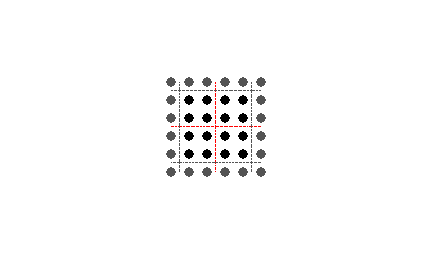
\includegraphics[width=\linewidth]{model_code_parallelization.png}
		\end{figure}
		\vspace{3cm}
		\Large
		\textbf{Paralelização MPI de métodos iterativos de resolução da equação de Poisson}
		
		\normalsize
		\vspace{0.5cm}
		Computação Paralela
		
		\vspace{1.5cm}
		\begin{tabular}{lr}
			Francisco Resende & 84767 \\
		\end{tabular}
		
		\vfill
		
		Departamento de Física\\
		\vspace{0.1cm}
		Universidade de Aveiro\\
		\vspace{0.1cm}
		03/07/2020
	\end{center}
\end{titlepage}

\pagenumbering{Roman}
\tableofcontents
\cleardoublepage

%\listoftables
\cleardoublepage

\listoffigures
\cleardoublepage

%\lstlistoflistings
\cleardoublepage

\pagenumbering{arabic}

\section{Introdução} \label{sec:Intro}
	
 De forma a tentar perceber o porquê de existir a necessidade de aplicar paralelização dos métodos iterativos que resolvem a equação de Poisson, é necessário entender o que é a equação de Poisson e como funcionam os métodos iterativos que a resolvem. A equação de Poisson é uma equação diferencial que é comummente utilizada em áreas como a eletrostática, física teórica e engenharia mecânica, a equação de Poisson usada para este trabalho pode ser representada pela equação \ref{eq:Poisson}.
 
 \begin{equation} \label{eq:Poisson}
 \frac{d^2V(x,y)}{dx^2}+\frac{d^2V(x,y)}{dy^2}=f(x,y)
 \end{equation}
		
onde

 \begin{equation} \label{eq:myF}
 f(x,y)=2-x^2-10y+50xy
 \end{equation}
 
Este tipo de equações de Poisson caracteriza-se, em 2D, como a soma das segundas derivadas parciais espaciais, sendo ela igual a uma função que depende das variáveis espaciais como se pode ver pela equação \ref{eq:Poisson} e pela equação \ref{eq:myF}.

Dentre os variados métodos iterativos usados para resolução de sistemas lineares, pode-se destacar os métodos de Jacobi e Gauss-Siedel. O método de Jacobi apesar de apresentar uma convergência relativamente lenta, tem um bom funcionamento para sistemas esparsos. No entanto, este método não se comporta bem para todos os casos, para obter um melhor desempenho este método requer que os elementos da diagonal principal sejam não nulos. Mas para que este método seja aplicado à equação diferencial é preciso realizar a sua discretização, para isso foi aplicada uma aproximação por diferenças finitas com um estêncil de 5 pontos, como podemos ver na equação \ref{eq:difFinit5Pts} e com um estêncil de 9 pontos como demonstrado na equação \ref{eq:difFinit9Pts}. Sendo esta aproximação um método de discretização, significa que transforma uma função contínua numa representação discreta, ou seja uma representação ponto a ponto.

  \begin{equation}  \label{eq:difFinit5Pts}
  V^{(k+1)}(i,j)=\frac{1}{4}[V^{(k)}(i-1,j)+V^{(k)}(i,j-1)+V^{(k)}(i,j+1)     	                +V^{(k)}(i+1,j)-h^2f(i,j)]
  \end{equation}
		
  \begin{equation}  \label{eq:difFinit9Pts}	
  \begin{aligned}
  V^{(k+1)}(i,j)=\frac{1}{20}[V^{(k)}(i-1,j-)+4V^{(k)}(i-1,j)+V^{(k)}(i-1,j+1)     	                +4V^{(k)}(i,j-1)\\+4V^{(k)}(i,j+1)+V^{(k)}(i+1,j-1)
                    +4V^{(k)}(i+1,j)+V^{(k)}(i+1,j+1)]\\-\frac{h^2}{40}[f(i-1,j)                                                                              	                +f(i,j-1)+8f(i,j)+f(i,j+1)+f(i+1,j)]
  \end{aligned}
  \end{equation}
  
O método de Gauss-Seidel, o segundo método usado neste trabalho, consiste num melhoramento do método de Jacobi que para calcular cada $V^{(k+1)}(i,1)$ usa a solução atual dos quatro vizinhos caso ela já tenha sido calculada, ou seja usa $V^{(k+1)}$ se j<i e $V^{(k+1)}$ se j>i. A expressão para este método pode ser representada pela equação \ref{eq:gaussSeidel}

  \begin{equation}  \label{eq:gaussSeidel}
   V^{(k+1)}(i,j)=\frac{1}{4}[V^{(k+1)}(i-1,j)+V^{(k+1)}(i,j-1)+V^{(k)}(i,j+1)     	                +V^{(k)}(i+1,j)-h^2f(i,j)]
  \end{equation}
		
Apesar do método usar valores calculados na iteração atual e outros da iteração anterior, os primeiros valores calculados de cada iteração irão usar valores da iteração passada. Se este último método não for associado a um outro método de auxilio, não irá funcionar quando num programa paralelizado.

Como é possível ver pelas equações \ref{eq:difFinit5Pts}, \ref{eq:difFinit9Pts} e \ref{eq:gaussSeidel} ambos os métodos percorrem todos os pontos do sistema o que faz com que o programa tenha uma complexidade de $n_x*n_y$, onde $n_x$ e $n_y$ são as dimensões do sistema. Como este tipo complexidade computacional aparece a necessidade de dividir o domínio global do sistema em subdomínios e para isso realizar a paralelização do programa. Neste trabalho a paralelização foi totalmente realizada em MPI. 

\pagebreak
		
\section{Divisão do domínio global em subdomínios} \label{sec:global2Local}
\label{sec:global2Local}
Para que os métodos possam ser implementados de forma paralela, o domínio global tem de ser dividido em subdomínios locais. Estes subdomínios locais estarão distribuídos por cada processo de forma a agilizar os cálculos dos métodos, como pode ser visto na figura \ref{fig:subDomains}.

  \begin{figure}[H]
  \centering
  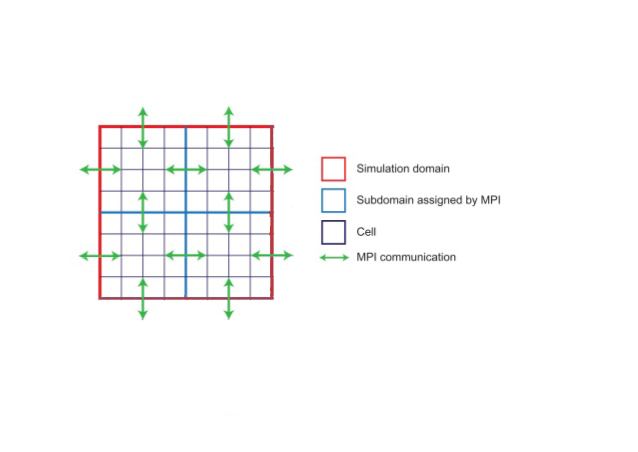
\includegraphics[width=\linewidth]{domain_decomposion_2.png}
  \caption{Decomposição do domínio}
  \label{fig:subDomains}
  \end{figure}

Como demonstra a figura \ref{fig:subDomains} o domínio é dividido pelos vários processos, mas mantendo comunicação com os diversos processos pois são necessários valores dos processos vizinhos de cada processo para que os valores das fronteira entre processos sejam calculados.

%\subsection{Sequential Addressing com Reverse Loop} \label{subsec:Sequential}



%\subsection{Interleaved Addressing com Strided Index} %\label{subsec:Interleaved}



%\subsection{Algoritmo de normalização}\label{subsec:Normalize}

\section{Criação de códigos de paralelização}

Tendo em conta o que foi falado na secção \ref{sec:global2Local} e o guião do trabalho, foram implementados códigos para escrita de resultados num ficheiro binário, um código que comportava condições fronteira diferentes, método de Jacobi que usava discretização com um estêncil de 9 pontos e um algoritmo que possibilitasse a implementação paralelizada do método de Gauss-Seidel.

\subsection{Escrita de resultados num ficheiro binário (alínea a)} \label{subsec:alineA}

A escrita de resultados tem de ser realizada assim que o método convergir, mas  nem todos os valores dos subdomínios podem ser escritos no ficheiro, visto que cada subdomínio comporta mais 2 linhas e 2 colunas. Estas linhas e colunas a mais servem para armazenar os valores das condições fronteira e ainda valores dos processos vizinhos que serão usados para cálculos. Tal como todos os valores não podem ser todos escritos, cada processo tem de saber em que parte do ficheiro irá escrever. De forma a resolver este último problema foi implementado um subarray que indicaria a cada processo onde escrever no ficheiro. Tendo em conta o constructor de um subarray, o array \textit{gsizes} foi inicializado com o tamanho do domínio global (\textit{$gsizes[0]=n_x$} e \textit{$gsizes[1]=n_y$}), o array \textit{lsizes} foi inicializado com  \textit{$lsizes[0]=myrows$} e \textit{$lsizes[1]=mycols+1$} (\textit{myrows} e \textit{mycols} contêm o número de linhas e colunas, respetivamente, em que o processo irá trabalhar), e o array \textit{$start\_indices$} com \textit{$start\_indices[0]= mytoprow+1$} e \textit{$start\_indices[1]=0$}. Mas estes valores iniciais não satisfazem todos os processos, por isso foram implementadas condições \textit{if} de forma a acertar alguns valores como pode ser visto nos pseudocódigos \ref{alg:if1}, \ref{alg:if2} e \ref{alg:if3}.
\linebreak
\linebreak
 \begin{algorithm}[H]
 \KwResult{\textit{$lsizes[0]=myrows+1$}}
 \If{\textit{newid}==0 or \textit{newid}==1 or \textit{newid}==numprocs-2 or \textit{newid}==numprocs-1}{
   $lsizes[0]=myrows+1$\;
   }
 
 \caption{Correção no \textit{$lsizes[0]$}}
 \label{alg:if1}
 \end{algorithm}
 
Este algorítmo \ref{alg:if1} trata dos processos que se encontram nos 4 cantos do domínio global, pois estes têm de escrever a linha que corresponde às condições de fronteira de cima e de baixo.  
 
\begin{algorithm}[H]
 \KwResult{\textit{$start\_indices[0]= mytoprow$}}
 \If{\textit{newid}==0 or \textit{newid}==1}{
   \textit{$start\_indices[0]= mytoprow$}\;
   }
 
 \caption{Correção no \textit{$start\_indices[0]$}}
 \label{alg:if2}
 \end{algorithm}
 
Este algorítmo \ref{alg:if2} trata dos processos de \textit{newid} 0 e 1, pois estes têm de começar a escrever a partir da linha que corresponde às condições de fronteira de cima, linha índice 0.  
 
 \begin{algorithm}[H]
 \KwResult{\textit{$start\_indices[1]$=0}}
 \If{\textit{newid}$\%2!=0$}{
   \textit{$start\_indices[1]= myleftcol+1$}\;
   }
   
 \caption{Correção no \textit{$start\_indices[1]$}}
 \label{alg:if3}
 \end{algorithm}
 
Este algorítmo \ref{alg:if3} trata dos processos de \textit{newid} ímpar, pois estes têm de começar a escrever a partir do índice myleftcol+1 devido ao índice  myleft col corresponder ao processo da esquerda no caso destes processos. 

Com esta preparação de arrays foi realizada a criação do subarray, aberto/criado o ficheiro binário e utilizado este subarray como \textit{file view} para cada processo. Após esta criação foi realizada a criação do subarray que irá especificar que dados dos subdomínios será escrito no ficheiro, inicializando \textit{memsizes} com o tamanho do do array local de cada processo (\textit{memsizes[0]=myrows+2} e \textit{memsizes[1]=mycols+2}), o array \textit{lsizes} é o mesmo do subarray anterior, e o array \textit{$start\_indices$} com \textit{$start\_indices[0]=1$} e \textit{$start\_indices[1]=newid\%2$}, pois só os processos com \textit{newid} par precisam de escrever a primeira coluna que corresponde à condição de fronteira da esquerda. Mas como os valores iniciais de \textit{$start\_indices$} não satisfazem todos os processos, foi implementada uma condição \textit{if} de forma a acertar estes valores como pode ser visto no pseudocódigo \ref{alg:if4}.

\begin{algorithm}[H]
 \KwResult{\textit{$start\_indices[0]= 0$}}
 \If{\textit{newid}==0 or \textit{newid}==1}{
   \textit{$start\_indices[0]= 0$}\;
   }
 
 \caption{Correção no \textit{$start\_indices[0]$}}
 \label{alg:if4}
 \end{algorithm}

Este algorítmo \ref{alg:if4} trata dos processos de \textit{newid} 0 e 1, pois estes têm de escrever a partir da linha 0 devido a essa linha conter os valores da condição fronteira de cima.

Após esta correção de valores o subarray foi criado e usado para realizar a escrita segundo o file view criado a partir do primeiro subarray.  

\pagebreak

\subsection{Alteração das condições fronteira (alínea b)}

Única e exclusivamente para esta alínea foi nos pedido para que usássemos as condições fronteira, $V(x=-1,y)=1y$, $V(x=+1,y)=\frac{5}{2}+\frac{y}{2}$, $V(x,y=-1)=\frac{1}{2}+\frac{3x}{2}$ e $V(x,y=+1)=2+x$. Esta alteração resumiu-se a trocar o código das condições fronteira desejadas.

Com estas condições fronteira foi obtida a representação gráfica que pode ser vista na figura \ref{fig:newCondFront} e comparado com a representação gráfica com as condições iniciais originas da figura XXX.

  \begin{figure}[H]
  \centering
  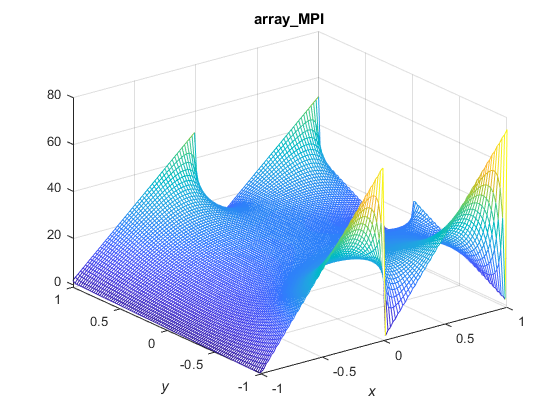
\includegraphics[width=\linewidth/2]{alineab.png}
  \caption{Representação gráfica com as novas condições fronteira para 4 processos e um domínio global de 100x100.}
  \label{fig:newCondFront}
  \end{figure}
  
  \begin{figure}[H]
  \centering
  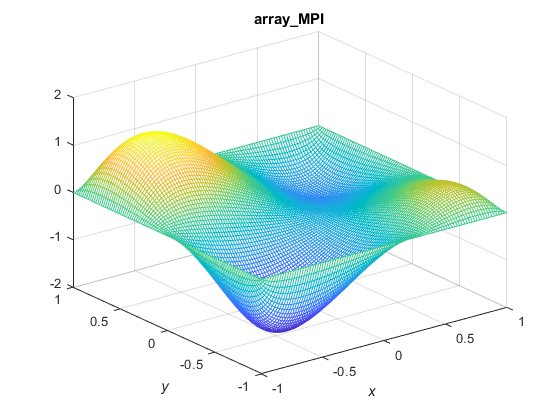
\includegraphics[width=\linewidth/2]{alineaa.png}
  \caption{Representação gráfica com as condições fronteira antigas para 4 processos e um domínio global de 100x100.}
  \label{fig:newCondFront}
  \end{figure}

\pagebreak

\subsection{Método de Jacobi com discretização com um estêncil de 9 pontos (alínea c)}

Com objetivo de diminuir os erros da discretização foi pedido para que utilizássemos um discretização com um estêncil de 9 pontos como o da equação \ref{eq:difFinit9Pts} da secção \ref{sec:Intro}. Para que este novo algorítmo funcionasse para todos os pontos dos subdomínios, cada processo tem de conhecer não só os processos vizinhos de cima, esquerda, baixo e direita, mas também os vizinhos das diagonais. Esta necessidade pode ser vista na figura \ref{fig:comunDiag}, onde a bola verde é o ponto que está a ser calculado, as bolas vermelhas os pontos comuns aos estêncil de 5 pontos e para quais as comunicações já estavam deitas, as bolas azuis os pontos novos que entram no estêncil de 9 pontos e dentro destas, a bola azul clara que faz parte de um processo do qual ainda não existia comunicação.

\begin{figure}[H]
  \centering
  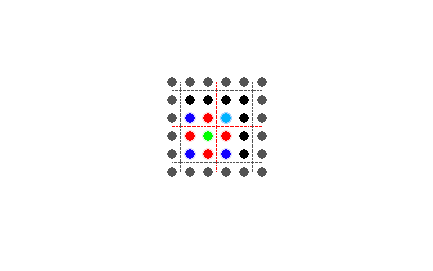
\includegraphics[width=\linewidth]{model_code_parallelization_alineac.png}
  \caption{Representação das comunicações necessárias para o algorítmo.}
  \label{fig:comunDiag}
  \end{figure}
  
A abordagem usada para encontrar os novos 4 vizinhos foi usado o comando \textit{$MPI\_Cart\_coords$} que baseado nos \textit{newids} do \textit{comm2d} devolve as coordenadas como se os processos estivessem distribuídos numa grelha, estas coordenadas são armazenadas na variável \textit{mycoords}. A partir destas coordenadas são calculadas as coordenadas dos 4 novos vizinhos (\textit{topleftcoords}, \textit{toprightcoords}, \textit{bottomrightcoords} e \textit{bottomleftcoords}), estes cálculos são realizados como os pseudocódigos \ref{alg:nbrtl}, \ref{alg:nbrtr}, \ref{alg:nbrbl} e \ref{alg:nbrbr}. Estes vizinhos são considerados por \textit{default} como \textit{$MPI\_PROC\_NULL$}.

\pagebreak

\begin{algorithm}[H]
 \KwResult{\textit{topleftcoords}}
 \If{\textit{newid}$\%2!=0$ and \textit{newid}!=1}{
   \textit{topleftcoords[0]}=\textit{mycoordscoords[0]}-1\;
      \textit{topleftcoords[1]}=\textit{mycoordscoords[1]}-1\;
   }
   
 \caption{Coordenadas do processo vizinho de cima da esquerda}
 \label{alg:nbrtl}
 \end{algorithm}
 
O pseudocódigo \ref{alg:nbrtl} calcula as coordenadas do vizinho de cima da esquerda para todos os processos excepto para os de \textit{newid} par e o processo 1, pois serão os únicos que não terão este vizinho.

\begin{algorithm}[H]
 \KwResult{\textit{toprightcoords}}
 \If{\textit{newid}$\%2==0$ and \textit{newid}!=0}{
   \textit{toprightcoords[0]}=\textit{mycoordscoords[0]}-1\;
      \textit{toprightcoords[1]}=\textit{mycoordscoords[1]}+1\;
   }
   
 \caption{Coordenadas do processo vizinho de cima da direita}
 \label{alg:nbrtr}
 \end{algorithm}
 
O pseudocódigo \ref{alg:nbrtr} calcula as coordenadas do vizinho de cima da direita para todos os processos excepto para os de \textit{newid} ímpar e o processo 0, pois serão os únicos que não terão este vizinho. 
 
 \begin{algorithm}[H]
 \KwResult{\textit{bottomleftcoords}}
 \If{\textit{newid}$\%2!=0$ and \textit{newid}!=numprocs-1}{
   \textit{bottomleftcoords[0]}=\textit{mycoordscoords[0]}+1\;
      \textit{bottomleftcoords[1]}=\textit{mycoordscoords[1]}-1\;
   }
   
 \caption{Coordenadas do processo vizinho de baixo da esquerda}
 \label{alg:nbrbl}
 \end{algorithm}
 
O pseudocódigo \ref{alg:nbrbl} calcula as coordenadas do vizinho de baixo da esquerda para todos os processos excepto para os de \textit{newid} par e o processo numprocs-1, pois serão os únicos que não terão este vizinho. 
 
 \begin{algorithm}[H]
 \KwResult{\textit{bottomrightcoords}}
 \If{\textit{newid}$\%2==0$ and \textit{newid}!=numprocs-2}{
   \textit{bottomrightcoords[0]}=\textit{mycoordscoords[0]}+1\;
      \textit{bottomrightcoords[1]}=\textit{mycoordscoords[1]}+1\;
   }
   
 \caption{Coordenadas do processo vizinho de baixo da direita}
 \label{alg:nbrbr}
 \end{algorithm}

O pseudocódigo \ref{alg:nbrbr} calcula as coordenadas do vizinho de baixo da direita para todos os processos excepto para os de \textit{newid} ímpar e o processo numprocs-2, pois serão os únicos que não terão este vizinho. 

Após a obtenção dos 4 novos vizinhos foi realizada a comunicação entre os mesmos e armazenado o valor do vizinho no canto do array local referente ao vizinho, como por exemplo \textit{mynew[myrows+1][mycols+1]} para o vizinho de  baixo da direita.

\pagebreak

\subsection{Método de Gauss-Seidel paralelizado (alínea d)}

Como é referido no guião, caso o programa não fosse paralelizado bastaria mudar o código referente à equação \ref{eq:difFinit5Pts} e trocar o código referente a $V^{k}$ e passar para $V^{k+1}$. Esta mudança pode ser realizada, pois como se pode ver pela figura \ref{fig:gaussSeidelNParalel} a partir do cálculo do ponto verde o método de Gauss-Seidel estará a seguir a equação \ref{eq:gaussSeidel}, a utilização unicamente de $V^{k+1}$ deve-se a dois fatores, um deles que inicialmente ambas as matrizes serem iguais e que no fim de cada iteração os valores da matriz $V^{k+1}$ são transferidos para $V^{k}$. Ao utilizarmos um programa paralelizado irá aparecer problemas nas fronteiras dos processos, como pode ser visto na figura \ref{fig:gaussSeidelParalel}.

\begin{figure}[H]
  \centering
  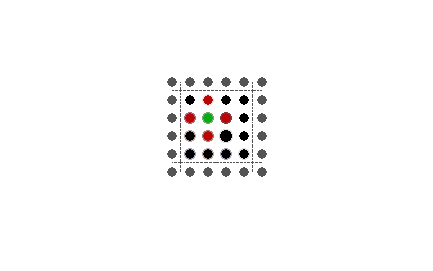
\includegraphics[width=\linewidth]{model_code_parallelization_nparalel_alinead.png}
  \caption{Gauss-Seidel num programa não paralelizado.}
  \label{fig:gaussSeidelNParalel}
  \end{figure}
\pagebreak
Na figura \ref{fig:gaussSeidelParalel} está a ser considerado que ambos os 4 processos estão em determinada iteração a calcular o ponto que corresponde à bola verde, em vermelho estão assinalados os pontos que seriam considerados "novos" e a azul os pontos considerados "antigos". Como é possível ver existem pontos que têm duas cores, o que faz com que a equação \ref{eq:gaussSeidel} não seja cumprida, ou seja não estaríamos perante o método de Gauss-Seidel.

\begin{figure}[H]
  \centering
  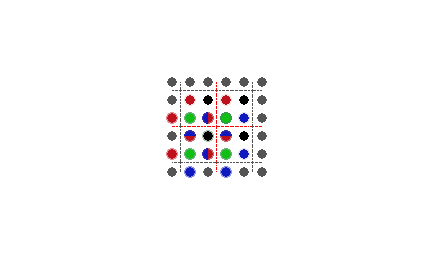
\includegraphics[width=\linewidth]{model_code_parallelization_alinead.png}
  \caption{Gauss-Seidel num programa paralelizado.}
  \label{fig:gaussSeidelParalel}
  \end{figure}

De forma a contornar este problema, foi nos pedido para implementarmos o método de Gauss-Seidel com uma atualização do tipo vermelho-preto. Este tipo de atualização consiste em "atribuir" a cor vermelho ou preto aos pontos de forma que os pontos vizinhos de um dado ponto tenham cor diferente desse mesmo ponto. Após esta "atribuição" são calculados os valores de todos os pontos pretos, é feita a comunicação desses novos valores com os vizinhos, por seguinte é calculado os valores dos pontos vermelhos (este cálculo já usa valores "novos") e no fim é comunicado as mudanças dos pontos vermelhos. 

Este tipo de atualização foi implementada como é mostrado nos pseudocódigos \ref{alg:blackpoints} e \ref{alg:redpoints}.

\begin{algorithm}[H]
 \KwResult{\textit{mynew} dos pontos pretos}
 \For{i=1;i<myrows+1;i++}{
   \For{$j=i\%2==0?2:1$;j<mycols+1;j+=2}{
     \textit{mynew[i][j]}=0.25*(\textit{mynew[i-1][j]}+\textit{mynew[i][j-1]}+\textit{mynew[i][j+1]}+\textit{mynew[i+1][j]}-$h^{2}$*myf[i][j])\;
   }
 }
 Comunicações\;
 \caption{Cálculos dos valores dos pontos pretos.}
 \label{alg:blackpoints}
 \end{algorithm}
 
O pseudocódigo \ref{alg:blackpoints} calcula os valores dos pontos pretos, irá percorrer todas as linhas e saltar as colunas com pontos vermelhos. Para que isto aconteça a primeira coluna será sempre a de índice 2 para linhas pares e a de índice 1 para linhas ímpares, o incremento realizado no índice das colunas é de 2. Após realizados os cálculos, são efetuadas as comunicações.

\begin{algorithm}[H]
 \KwResult{\textit{mynew} dos pontos pretos}
 \For{i=1;i<myrows+1;i++}{
   \For{$j=i\%2==0?1:2$;j<mycols+1;j+=2}{
     \textit{mynew[i][j]}=0.25*(\textit{mynew[i-1][j]}+\textit{mynew[i][j-1]}+\textit{mynew[i][j+1]}+\textit{mynew[i+1][j]}-$h^{2}$*myf[i][j])\;
   }
 }
 Comunicações\;
 \caption{Cálculos dos valores dos pontos vermelhos.}
 \label{alg:redpoints}
 \end{algorithm}

O pseudocódigo \ref{alg:redpoints} calcula os valores dos pontos vermelhos, irá percorrer todas as linhas e saltar as colunas com pontos pretos. Para que isto aconteça a primeira coluna será sempre a de índice 1 para linhas pares e a de índice 2 para linhas ímpares, o incremento realizado no índice das colunas é de 2. Após realizados os cálculos, são efetuadas as comunicações.

Após estas implementações o algorítmo de Gauss-Seidel pode ser usado em programas paralelizados.

\section{Conclusão}

Após as implementações e testes realizados, posso concluir que a maior diferença notada foi no número de iterações necessárias para que o método convirja. O algoritmo do esquema de atualização alternativo, vermelho-preto, poderia ser melhorado visto que as comunicações são de linhas e colunas completas, ou seja existem dados que serão repetidos e escritos no mesmo local.
As maiores dificuldades enfrentadas neste trabalho residiram em tentar conjugar o MPI com os algorítmos que idealizava. Apesar das dificuldades enfrentadas penso que este trabalha contempla tópicos bastante interessantes e úteis às necessidades do quotidiano.

\end{document}